\documentclass{article}
\usepackage{neurips_2019}

\usepackage[utf8]{inputenc} % allow utf-8 input
\usepackage[T1]{fontenc}    % use 8-bit T1 fonts
\usepackage[usenames, svgnames]{xcolor}
\usepackage{hyperref}       % hyperlinks
\usepackage{bchart}
\usepackage{pgfplots}
\pgfplotsset{width=7 cm,compat=1.5}
\hypersetup{
	colorlinks=true,
	linkcolor={red!80!black},
	%	citecolor={blue!80!black},
	%	urlcolor={magenta}
}

\usepackage{url}            % simple URL typesetting
\usepackage{booktabs}       % professional-quality tables
\usepackage{amsfonts}       % blackboard math symbols
\usepackage{nicefrac}       % compact symbols for 1/2, etc.
\usepackage{microtype}      % microtypography
\usepackage{subcaption}
\usepackage{graphicx}

% Useful packages
\usepackage{amsmath, amssymb, amsfonts, bm}
\usepackage{amsthm}
\usepackage{mathtools}
%\usepackage[usenames, dvipsnames]{color}
\usepackage{cleveref}
\crefname{figure}{Figure}{Figures}
\crefname{table}{Table}{Tables}

\usepackage{enumitem}
\setlist{leftmargin=*} 
%\setlist[enumerate]{labelindent=5pt, label=\alph*)} 

\usepackage{wrapfig}
\usepackage{tabularx}
\usepackage{adjustbox}


% \usepackage{blindtext}

\newtheorem{theorem}{Theorem}
\newtheorem{proposition}[theorem]{Proposition}
\newtheorem{corollary}[theorem]{Corollary}
\newtheorem{lemma}[theorem]{Lemma}
\newtheorem{remark}[theorem]{Remark}

\theoremstyle{remark}
\newtheorem*{notation}{Notation}
%\newtheorem*{remark}{Remark}
\newtheorem*{note}{Note}

\theoremstyle{definition}
\newtheorem{definition}[theorem]{Definition}
\newtheorem{fact}{Fact}
\newtheorem*{observation}{Observation}
\newtheorem*{condition}{Condition}
\newtheorem*{claim}{Claim}
\newtheorem*{example}{Example}
\newtheorem*{question}{Question}


\newcommand{\colorbx}[1]{\medskip\noindent\scalebox{1.05}{\fcolorbox{SaddleBrown}{white}{\color{SteelBlue}{\textbf{#1}}}}}

\newcommand{\tk}[1]{\textcolor{red}{TK: #1}}
\newcommand{\ao}[1]{\textcolor{green}{AO: #1}}
\newcommand{\tsj}[1]{\textcolor{magenta}{TSJ: #1}}
\newcommand{\va}[1]{\textcolor{blue}{Vincent A: #1}}

\newcommand{\Reals}{\mathbb{R}}
\newcommand{\T}{\mathsf{T}}
\DeclareMathOperator{\softmax}{\mathrm{softmax}}

\newcommand{\cA}{\mathcal{A}}
\newcommand{\cG}{\mathcal{G}}
\newcommand{\cK}{\mathcal{K}}
\newcommand{\cH}{\mathcal{H}}
\newcommand{\cI}{\mathcal{I}}

\newcommand{\vect}[1]{\mathbf{#1}}
\newcommand{\vx}{\vect{x}}
\newcommand{\vy}{\vect{y}}
\newcommand{\vone}{\vect{1}}
\newcommand{\proj}{\mathrm{proj}}

\newcommand{\imatch}{g^{\mathrm{v}}}
\newcommand{\mmatch}{g^{\mathrm{m}}}

\newcommand{\doadd}{h^{\mathrm{a}}}
\newcommand{\doreplace}{h^{\mathrm{r}}}

\newcommand{\tlast}{\tau^{\mathrm{last}}}
\newcommand{\tlatest}{\tau^{\mathrm{latest}}}
\newcommand{\tnow}{\tau^{\mathrm{now}}}
\newcommand{\tnone}{\tau^{\mathrm{none}}}

\newcommand{\rhead}{rh}
\newcommand{\whead}{wh}


\title{Learning Multi-Step Spatio-Temporal Reasoning with Selective Attention Memory Network}

\author{T.S. Jayram, Tomasz Kornuta, Vincent Albouy, Emre Sevgen, Ahmet Ozcan}

\begin{document}
\maketitle
\begin{abstract}
Visual reasoning in videos requires understanding temporal concepts in addition to the objects and their relations in a given frame.  
%Selective attention and memory are the essential faculties, which humans rely on to accomplish this task.  
%In analogy with human reasoning, we present Selective Attention Memory Network (SAMNet), an end-to-end differentiable recurrent 
%model equipped with external memory.  
To that end,
we present Selective Attention Memory Network (SAMNet), an end-to-end differentiable recurrent 
model equipped with external memory.  
In analogy with human reasoning, 
SAMNet can perform multi-step reasoning on a frame-by-frame basis, and dynamically control information flow to the memory 
to store context-relevant representations and from the memory to answer questions. 
We tested our model on the COG dataset (a multi-frame visual question answering test).
SAMNet outperforms the the original COG model, 
especially on the hardest version of the dataset with longer sequences and a maximum number of distractors.
We also demonstrate that our model has extraordinary generalization capabilities going from easy to hard tasks, without and with additional fine-tuning.
%, and outperformed the state of the art baseline for hard tasks and in terms of generalization over video length and scene complexity.
%	We introduce the Selective Attention Memory Network (SAMNet), a end-to-end differentiable architecture for video reasoning. It is a recurrent model with an external memory that enables frame by frame reasoning over text and video. 
%		We show SAMNet's abilities on the COG dataset made for Video Question Answering (Guangyu Robert Yang, Igor Ganichev et al., ECCV 2018). 
\end{abstract}

\section{Introduction}

Integration of vision and language in deep neural network models allows the system to learn joint representations of objects, concepts, and relations.  Potentially, this approach can address Harnad's "symbol grounding problem" \cite{harnad2003symbol} and lead to visually grounded language learning.
%In addition to multimodal learning, visual grounding of language is another opportunity that the AI community is excited about, especially in the context of Harnad's "symbol grounding problem" \cite{harnad2003symbol}. 

Starting with the Visual Question Answering (VQA) dataset \cite{}, many tasks that integrate vision and language have emerged in the past several years\cite{mogadala2019trends}.  As a departure from the simpler vision tasks like classification and object detection, visual reasoning has become the core emphasis in these tasks. Visual reasoning mainly deals with the comparison of object attributes, counting and other relational questions.

In contrast to VQA, which comes with static image and question pairs, another emerging direction is Video QA \cite{}, which introduces the aspect of time.  In addition to spatial reasoning, video input provides an opportunity to work on temporal relations and reasoning.  As evident from human cognition, attention and memory are the key competencies required to solve these problems, and unsurprisingly, the AI research is rapidly growing in these areas.

The ability to deal with time can pose a challenge for natural language processing (NLP) as well; for instance, in question answering (QA) and dialog applications.  The current NLP solutions, in certain problem settings, can work around this challenge by processing the entire text input and reason over it multiple times using attention \cite{vaswani2017attention} or other mechanisms. For example, solutions to the bAbI reasoning task (e.g. Memory Networks \cite{weston2015towards}), typically involve processing the supporting facts all at once, which reside in memory and available to provide answers. Similarly, in Visual Dialog~\cite{das2017visual} the system keeps the whole history of the dialog in memory.  In real-time dialog or video QA, there may not be such an opportunity to have the question and entire input all at once in the beginning.  

Video reasoning datasets such as SVQA (Synthetic Video Question Answering)~\cite{song2018explore} and COG \cite{yang2018dataset} have limited number of frames (e.g. 4-16 frames), and therefore manageable by the neural net models to process and represent all of the visual information.  As an example, according to\cite{song2018explore} the authors extracted visual features from each frame and aggregated features of all clips from one video to form a sequential video representation.
These solutions may demonstrate high accuracy, however, generalization to arbitrary length video sequences will be problematic.  Such approaches also differ from the human cognitive strategies.  Humans have the ability to selectively pay attention and store salient items or events in memory based on their goals.  Working memory and episodic memory systems are responsible for this remarkable ability. 

%Fluid Intelligence:
%
%IQ may be viewed as a composite comprising multiple elements: In many theories of intelligence, a distinction is made between fluid and crystallized intelligence (8). Fluid intelligence comprises the set of abilities involved in coping with novel environments and especially in abstract reasoning; crystallized intelligence is the product of the application of these processes. Fluid intelligence is often measured by tests such as figural analogy, classification, and matrix problems, whereas crystallized intelligence is measured by tests of vocabulary and general information (9). 
%~\cite{sternberg2008increasing}
%
%Cognitively, gF is thought to be related to metacognition6(knowing about and reflecting upon one’s own ongoing mentalprocesses) and to working memory4,5,7–9(the active maintenanceof domain-specific information plus domain-general attention-al or ‘executive’ control of ongoing processing). One componentof attentional control is the ability to overcome interference thatwould otherwise disrupt performance by compromising taskgoals or information held active in working memory. Individualdifferences in gF are most pronounced in behavioral measureswhen attentional control is required4,8,10. For this reason, gF isthought to be related to attentional control specifically~\cite{gray2003neural}


%In recent years there has been substantial progress in systems  that  can  find  factual  answers  in  text,  starting  with IBM’s Watson system~\cite{ferrucci2010building}, and now with high-performing neural systems that can answer short questions provided they are given a text that contains the answer e.g.~\cite{wang2018glue}
%
%
%AI  has  achieved  remarkable  mastery  over  games  such  asChess, Go, and Poker, and evenJeopardy!, but the rich variety of standardized exams has remained a landmark chal-lenge.   Even  in  2016,  the  best  AI  system  achieved  merely 59.3\% on an 8th Grade science exam challenge (Schoenicket al., 2016).
%
%Playing Atari Games~\cite{mnih2015human}
%
%
%Despite several successes across many domains Deep learning~\cite{lecun2015deep} still struggles with
%
%learning algoritms
%learning reasoning~\cite{graves2016hybrid}
%
%
%Wingrad Scheme challenge~\cite{levesque2012winograd}

%visual reasoning~\cite{mogadala2019trends} - datasets such as COG~\cite{yang2018dataset} and 
%SVQA (Synthetic Video Question Answering)~\cite{song2018explore}
%
%
%ARISTO project~\cite{clark2019f} - based on RoBERTa~\cite{liu2019roberta} contextual word embeddings
%
%transformer-based solutions~\cite{vaswani2017attention} using self-attention
%
%
%“The current neural network approaches will find it difficult to determine which combinations of ‘later’, ‘earlier’, ‘more’, and ‘less’ constitute ‘increase’ and which constitute ‘decrease,'” Davis says. “Neural networks have no inherent idea of magnitude or of time.”
%~\cite{davis2016write}





%\begin{itemize}
%\item bAbI:  MemNets~\cite{weston2014memory} have access to the whole story at once
%\item the same goes to SoftPats~\cite{haurilet2019s} - they build graph per frame and then frame number is treated as one dimensions, so at the end the \textit{Traveler} can access all of them at the same time 
%\item The paper~\cite{le2019learning} focuses on SVQA and TGIF-QA -  they access all frames at once, i.e. cut the video into clips, process each frame with CNNs and then aggregate feature representations of equal-size clips obtained by a temporal attention mechanism. So in fact the model has access to all frames all the time.
%\end{itemize}
%so the time aspect is really... not dealt with?
%
%Additionally, in~\cite{song2018explore} the authors introduced a large-scale dataset caled SVQA (Synthetic Video Question Answering) consisting of (Total QA pairs: 83160/11760/23760 and Total Videos 8400/1200/2400).
%As "using all frames is time-consuming. Thus we divide each video into clips (segments) of 16 frames, with 80\% overlap between successive clips (segments)" and "We extract feature from each clip and aggregate features of all clips from one video to form a sequential video representation." -- which means that they identified the problem that you "cannot extract features from all frames" at the beginning and pass that to the model. But instead of proposing a solution that will deal with the video on per-frame basis, they "cheated". ;)
%
%IMPORTANT: \textbf{we do not have any explicit assumptions when it comes to number of frames/length of the movie/number of distractionts}, so there is no need for cutting video into cuts etc.

\subsection{Contributions}
This work have attempted to address the issues mentioned above and propose a new model that can dynamically process video input frame-by-frame, reason over images and remember the salient concepts to answer questions.  We have tested this model on the COG dataset \cite{yang2018dataset} and compared to the baseline results.  Our results indicate that the model is capable of:
%\begin{itemize}
%\item \textbf{Time aspect}:
\begin{itemize}
\item Learning the temporal association - grounding the time-related words with meaning
%\item Learning the concept of time
%\item time context being by-product of gates
%\end{itemize}

\item Learning complex, multi-step reasoning that involves grounding of words and visual representations of objects/attributes
%\begin{itemize}
%\item Learning complex, multi-step reasoning that involves grounding of words and visual representations/objects
\item Selectively control the flow of information to and from the memory to answer questions
%\end{itemize}
%\item \textbf{Selective Attention Memory}:
%\begin{itemize}
\item Updating the memory content only with relevant visual information depending on the temporal context
%\item content based and location based addressing for reading and writing
%\item new memory interface/gating designed in such a way enabling the model to control the flow of current visual information and content of the memory in a selective way

\end{itemize}
%\end{itemize}









\section{Model}

Selective Attention Memory Network (SAMNet) is a end-to-end differentiable model made for video reasoning. It is a model based on attention mechanisms but also on a Selective Attention Memory which is able to store selected entities. This memory enables SAMNet to reason across multiple frames and perform spatio-temporal reasoning. 
The core of SAMNet is based a recurrent cell called SAMCell. By aligning together a series of k SAMCells per frame, the network can perform k reasoning steps over a frame. At every new frame, a new series of k SAMCells is initiated. The SAMCell can read and write to memory at every frame using a content addressable mechanism. This section describes the model and the different units that composed a SAMCell. They are called the Question-driven Controller, the Visual Retrieval Unit, the Memory Retrieval Unit, the Reasoning unit, the Memory update unit, and the Summary Object Udpate Unit. 
The model is also composed of an Image Encoder and a Question Encoder both responsible to pre-process the visual and textual inputs. The output unit is a classifier.
All those modules are described below.

\subsection{Question-driven Controller}

The Question-driven Controller plays an important role in the reasoning process.
it drives the attention over the question and produces the new control states. Each new control state defines a new reasoning operation. The inputs of this unit are the past control state, the question encoding and the contextual words (see Question Encoding Unit). It uses the dot product attention between the contextual words
and the combination of the past control states and the question encoding.  This attention layer produces the new control state.

This unit also output the temporal class weights that will be used in the Reasoning Unit. It gives access to a temporal information for the current words. (last,latest,now, none temporal)

\subsection{Visual Retrieval Unit}

The visual retrievial unit is responsible to extract visual information from the current image given a control state coming from the Question-driven Controller. It is first projecting the past summary object and the feature maps together using the interaction module.
It is then using the attention module as follow. The query are the control states and the keys and are the feature maps coming from the image encoder. The results of this attention is applied on the modified features maps coming from the interaction module.  
This unit outputs the extracted object and the visual attention.

\subsection{Memory Retrieval Unit}

The role of the memory retrievial unit is to read and extract object from memory (Selective AttentionMemory).
As the Visual Retrievial Unit, it uses a combination of two following submodules. The interaction module responsible to blend the extracted object and the content of the memory. The attention module then extract the corresponding object in memory if present.


\subsection{Reasoning Unit}
\subsection{Memory update Unit}
\subsection{Summary Object Udpate Unit}

The image encoder, question encoder and output unit are described in the appendix.


\section{Experiments}

We evaluated SAMNet on the COG dataset~\cite{yang2018dataset}.
Our experiments were designed to study SAMNet's performance as well as its generalization abilities in different settings.
For this purpose, we used two different variants of the COG dataset: an easy one (Canonical) and a Hard version to explore a wide range of difficulties.
The main differences are the number of frames in the input sequence (4 vs. 8) and the maximum number of distractors (i.e., objects not relevant for the answer) per frame (1 vs. 10).
%More details on the dataset, its variants and tasks can be found in the Appendix.


%
%We compare our model to the original COG model  ~\cite{yang2018dataset} using their implementation (https://github.com/google/cog) and scores given by the authors. We also use the exact same training parameters detailed in the original paper.
%
%On the other side we trained SAMNet using IBM's Mi-Prometheus~\cite{kornuta2018accelerating}, a framework for research based on Pytorch. We trained all our models using NVIDIA’s GeForce GTX TITAN X GPUs. We trained  SAMNet using 8 reasoning steps SAMCells and a hidden state size of 128. The external memory has 128-bit slots. We trained our model until convergence but we also have set a training time limit of 80 hours.


\begin{figure}[htbp]
	\centering
  \begin{subfigure}{\textwidth}
    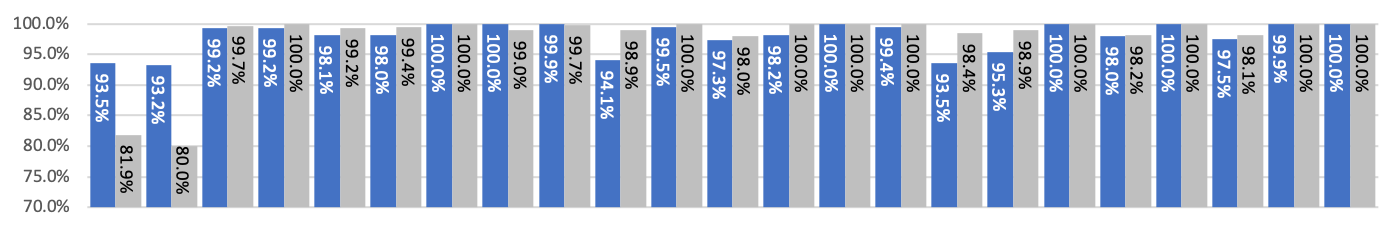
\includegraphics[width=0.92\textwidth]{../results/samnet_cog_orig_canonical_no_labels.png}
  \end{subfigure}%
  \newline
  \begin{subfigure}{\textwidth}
	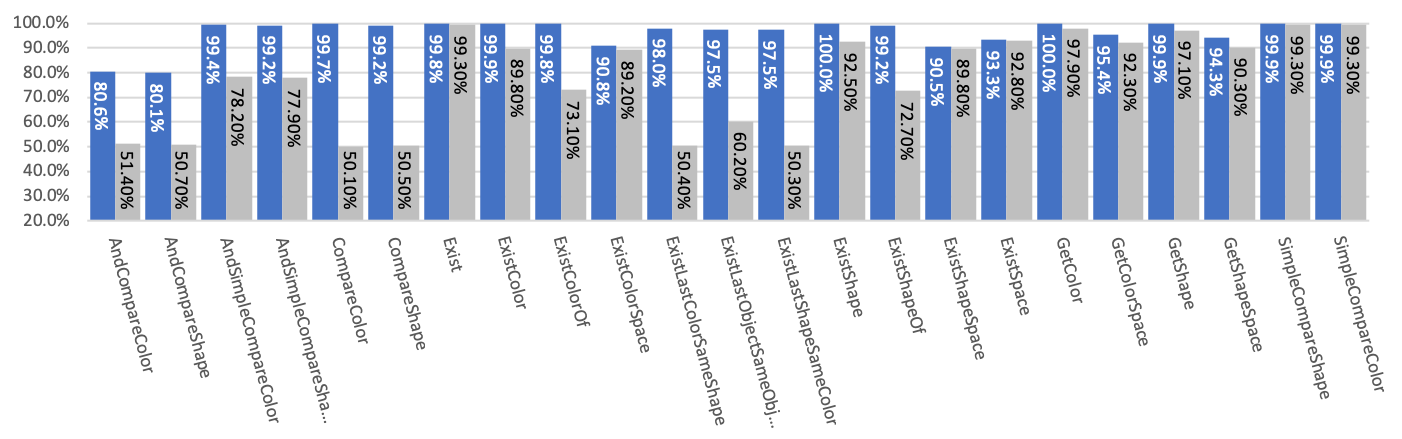
\includegraphics[width=0.93\textwidth]{../results/samnet_cog_orig_hard.png}
  \end{subfigure}%
\caption{Comparison of test set accuracies of SAMNet (blue) with original results achieved by the COG model (gray) on Canonical (top) and Hard (bottom) variants of the COG dataset.}
\label{fig:samnet_cog_detailed}
\end{figure}

\begin{figure}
	\centering
	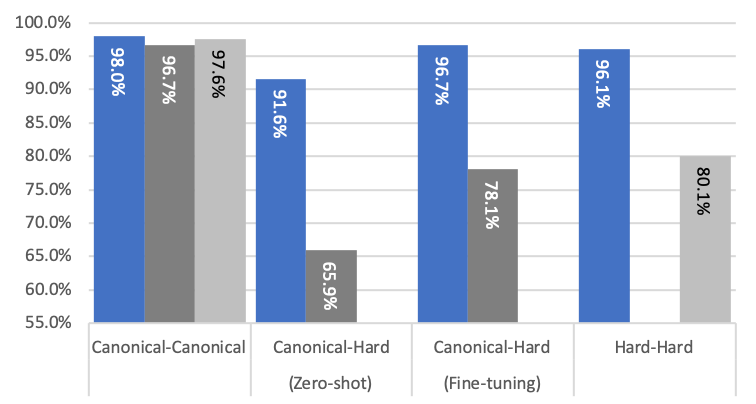
\includegraphics[width=0.75\textwidth]{../results/samnet_cog_overall_transfer.png}
	\caption{Total accuracies of SAMNet (blue) and COG models (light/dark gray) when testing generalization from Canonical to Hard variants of the dataset.}
	\label{fig:samnet_cog_overall_transfer}
\end{figure}

We have implemented and trained our SAMNet model using MI-Prometheus~\cite{kornuta2018accelerating}, a framework based on Pytorch~\cite{paszke2017automatic}. 
In our experiments, we have focused on 22 classification tasks and compared our results with the baseline model, as presented in \cref{fig:samnet_cog_detailed}.
For the Canonical variant (top row), we have achieved similar accuracies for the majority of tasks (with the total average accuracy of 98.0\% in comparison of 97.6\% achieved by the COG model), with significant improvements (around 13 points) for \textit{AndCompare} tasks.
As those tasks focus on compositional questions referring to two objects, we hypothesize that our model achieved better accuracy due to the ability to selectively pick and store the relevant objects from the past frames in the memory.
Despite there being some tasks in which our model reached slightly lower accuracies,
% (between 0.2 and 1.8 points)
when comparing performances on the Hard variant, it improves upon the  COG baseline on all tasks, with improvements varying from 0.5 to more than 30 points.

The goal of the next set of experiments was to test the generalization ability concerning the sequence length and number of distractors.
For that purpose, we have compared the accuracies of both models when trained on the Canonical variant and tested on Hard (\cref{fig:samnet_cog_overall_transfer}).
As the original paper does not include such experiments, we have performed them on our own.  The light gray color indicates the original results, whereas dark gray indicates the accuracies of COG models that we have trained (fine-tuning/testing) using the original code provided by the authors.
For sanity check, in the first column, we report both the best-achieved score and the score reported in the paper when training and testing on Canonical variant, without any fine-tuning.
In a pure \textit{transfer learning} setup (second column), our model shows enormous generalization ability, reaching 91.6\% accuracy on the test set.
We have also tested both models in a setup where the model trained on a Canonical variant underwent additional fine-tuning (for a single epoch) on the Hard variant (third column).
In this case, the SAMNet model also reached much better performance, and, interestingly, achieved better scores from the model trained and tested exclusively on the Hard variant.
In summary, the results clearly indicate that the mechanisms introduced in SAMNet  enable it to learn to operate independently of the total number of frames or number of distractions, and allow it to generalize to longer videos and more complex scenes. One other strength of SAMNet is its interpretability. Observing attention maps (see supplementary material) shows that SAMNet can effectively perform multi-step reasoning over questions and frames as intended. It also accurately classifies temporal contexts as designed. However we notice that the model can sometime discover alternative strategies that were not in the intended design but the answers are still correct. 

%we used the canonical (easy) and hard settings that alter the number of distractors and sequence length.  Since there was no baseline for these tests (train on canonical, test on hard), we ran our own experiments using the COG model provided by the authors.  SAMNet achieves the highest overall scores for all categories of experiments (\cref{fig:samnet_cog_overall_transfer}), especially for the tests run on the hard dataset.  Among the 22 classification tasks, we highlighted the two most difficult tasks that affect the overall score. 
%We argue that the generalization capability of SAMNet is mainly due to the dynamic frame-by-frame processing of the input sequence. 
%The mechanisms introduced in SAMCell learn to operate independently of the total number of frames and allow to generalize to longer video lengths.
%As shown in \cref{fig:samnet_cog_overall_transfer}, when trained on the easy dataset, SAMNet still performs 91.6\% when tested on the hard dataset, whereas COG drops from 97.6\% to 65.9\%   The visualization of the trained SAMNet model (see Appendix) indicates that the model learns the concept of time, helping it to control the flow of information from visual input to the memory.  Therefore, the memory is updated efficiently instead of storing all information across all frames.







\section{Summary}

\section*{Acknowledgement}
The authors would like to thank to the authors of COG paper (Igor Ganichev in particular) for sharing the detailed results with performances achieved by their COG baseline model.
	
%\newpage
\bibliographystyle{abbrv}
\bibliography{../cog_bibliography}

\newpage
\appendix

\section{Description of datasets}

Most of the VQA datasets have strong biases. This allow models to learn strategies without reasoning about the visual input~\cite{Santoro2017ASN}.
The CLEVR dataset~\cite{johnson2017clevr} was developed to address those issues and come back to the core challenge of visual QA which is testing reasoning abilities.
CLEVR contains images of 3D-rendered objects; each image comes with a number of highly compositional questions that fall into different categories.
Those categories fall into 5 classes of tasks: Exist, Count, Compare Integer, Query Attribute and Compare Attribute. 
The CLEVR dataset consists of:
\begin{itemize}
\item 	A training set of 70k images and 700k questions,
\item	A validation set of 15k images and 150k questions,
\item	A test  set of 15k images and 150k questions about objects,
\item	Answers, scene graphs and functional programs for all train and val images and questions.
\end{itemize}
Each object present in the scene, aside of position, is characterized by a set of four attributes:
\begin{itemize}
\item 2 sizes: large, small,
\item 3 shapes: square, cylinder, sphere,
\item 2 material types: rubber, metal,
\item 8 color types: gray, blue, brown, yellow, red, green, purple, cyan,
\end{itemize}
resulting in 96 unique combinations.

Along with CLEVR, the authors~\cite{johnson2017clevr} introduced  CLEVR-CoGenT (Compositional Generalization Test, CoGenT in short), with a goal of evaluating how well the models can generalize, learn relations and compositional concepts.
This dataset is generated in the same way as CLEVR with two additional conditions.
As shown in \tableref{tab:cogent_conditions}, in Condition A all cubes are gray, blue, brown, or yellow, whereas all cylinders are red, green, purple, or cyan; in Condition B cubes and cylinders swap color palettes.
For both conditions spheres can be any colors.


The CoGenT dataset contains:
\begin{itemize}
\item	Training set of 70,000 images and 699,960 questions in Condition A,
\item	Validation set of 15,000 images and 149,991 questions in Condition A,
\item	Test set of 15,000 images and 149,980 questions in Condition A (without answers),
\item	Validation set of 15,000 images and 150,000 questions in Condition B,
\item	Test set of 15,000 images and 149,992 questions in Condition B (without answers),
\item	Answers, scene graphs and functional programs for all training and validation images and questions.
\end{itemize}

\begin{table}[h!]
	\centering
	\begin{tabular}{cccc}
		\toprule
		Dataset        & Cubes              & Cylinders &  Spheres         \\
		\midrule
		CLEVR   &  any color &  any color        &    any color    \\
		%\midrule
		CLEVR CoGenT A & gray / blue / brown / yellow  & red / green / purple / cyan       &    any color  \\
		CLEVR CoGenT B  & red / green / purple / cyan &   gray / blue / brown / yellow       &      any color  \\
		\bottomrule
	\end{tabular}
	\caption{Colors/shapes combinations present in CLEVR, CoGenT-A and CoGenT-B datasets}
	\label{tab:cogent_conditions}
\end{table}

 
 \newpage
\section{Full MAC and S-MAC comparison}

In \tableref{tab:results_full} we present the full comparison between MAC and S-MAC models.


\begin{table}[!h]
	\caption{CLEVR \& CoGenT accuracies for the MAC \& S-MAC models}
	\centering
	\begin{tabular}{ccccCcCc}
		\toprule
		\multirow{2}{*}{Model} & \multicolumn{3}{c}{Training} &  \multicolumn{2}{c}{Fine-tuning} &  \multicolumn{2}{c}{Test} \\
		\cmidrule{2-4} \cmidrule{5-6} \cmidrule{7-8} 
		& Dataset                & Time [h:m] & Acc [\%]          & Dataset & Acc [\%]  & Dataset & Acc [\%] \\
		\midrule
		\multirow{15}{*}{MAC} & \multirow{10}{*}{CLEVR}  & \multirow{10}{*}{30:52}  & \multirow{10}{*}{96.70} & \multirow{4}{*}{--}   & \multirow{4}{*}{--}  & CLEVR    & 96.17          \\
		\cmidrule{7-8} 
		&                        &  &               &     &                                & CoGenT-A    &  96.22   \\
		\cmidrule{7-8} 
		&                        &   &              &     &                               & CoGenT-B   & 96.27  \\
		
		\cmidrule{5-6} \cmidrule{7-8} 
		&                             &                                         &    &   \multirow{2}{*}{CoGenT-A}         &       \multirow{2}{*}{98.06}          & CoGenT-A &  94.60	         \\
		\cmidrule{7-8} 
		&                             &                                         &       &         &                & CoGenT-B &    93.28       \\
		\cmidrule{5-6} \cmidrule{7-8} 
		&                             &                                         &    &   \multirow{2}{*}{CoGenT-B}         &       \multirow{2}{*}{98.16}          & CoGenT-A &  93.02         \\
		\cmidrule{7-8} 
		&                             &                                         &       &         &                & CoGenT-B &    94.44       \\  
		
		\cmidrule{2-4} \cmidrule{5-6} \cmidrule{7-8} 
		& \multirow{5}{*}{CoGenT-A} & \multirow{5}{*}{30:52}     & \multirow{5}{*}{97.02}   &  \multirow{2}{*}{--}  &  \multirow{2}{*}{--}    & CoGenT-A & 96.88         \\
		\cmidrule{7-8} 
		&                             &                                         &       &         &                & CoGenT-B & 79.54          \\
		\cmidrule{5-6} \cmidrule{7-8} 
		&                             &                                         &    &   \multirow{2}{*}{CoGenT-B}         &       \multirow{2}{*}{97.91}          & CoGenT-A &  92.06         \\
		\cmidrule{7-8} 
		&                             &                                         &       &         &                & CoGenT-B &    95.62       \\
		\midrule
		\multirow{15}{*}{S-MAC} & \multirow{10}{*}{CLEVR}  & \multirow{10}{*}{28:30}  & \multirow{10}{*}{95.82} & \multirow{3}{*}{--}   & \multirow{3}{*}{--}  & CLEVR    & 95.29           \\
		\cmidrule{7-8} 
		&                        &  &               &     &                                & CoGenT-A    &  95.47   \\
		\cmidrule{7-8} 
		&                        &   &              &     &                               & CoGenT-B   &  95.58  \\		
		
		\cmidrule{5-6} \cmidrule{7-8} 
		&                             &                                         &    &   \multirow{2}{*}{CoGenT-A}         &       \multirow{2}{*}{97.48}          & CoGenT-A &  93.44         \\
		\cmidrule{7-8} 
		&                             &                                         &       &         &                & CoGenT-B &    92.31       \\
		\cmidrule{5-6} \cmidrule{7-8} 
		&                             &                                         &    &   \multirow{2}{*}{CoGenT-B}         &       \multirow{2}{*}{97.67}          & CoGenT-A &  92.11         \\
		\cmidrule{7-8} 
		&                             &                                         &       &         &                & CoGenT-B &    92.95       \\  		
		
		\cmidrule{2-4} \cmidrule{5-6} \cmidrule{7-8} 
		& \multirow{5}{*}{CoGenT-A}   & \multirow{5}{*}{28:33}   & \multirow{5}{*}{96.09}  &  \multirow{2}{*}{--}  &  \multirow{2}{*}{--}   & CoGenT-A & 95.91          \\
		\cmidrule{7-8} 
		&                             &                                         &     &          &                & CogenT-B & 78.71          \\
		\cmidrule{5-6} \cmidrule{7-8} 
		&                             &                                         &    &   \multirow{2}{*}{CoGenT-B}         &       \multirow{2}{*}{96.85}          & CoGenT-A &  91.24         \\
		\cmidrule{7-8} 
		&                             &                                         &       &         &                & CoGenT-B &    94.55       \\
		\bottomrule
	\end{tabular}
	\label{tab:results_full}
\end{table}

\section{Comparison of generalization capabilities}

In this section we present comparison of our results on generalization capabilities with selected state-of-the-art models.
In particular, we focused on three papers reporting state-of-the-art accuracies, i.e. PG+EE~\cite{johnson2017inferring} FiLM~\cite{perez2017film} and TbD~\cite{mascharka2018transparency}.
Deeper analysis of the papers revealed that it is most probable that different authors used different sets for reporting the scores, which questions the correctness of the comparison.
We find that the problems result from the fact that answers for the test sets aren't provided along with those sets, thus researchers started to use subsets of the validation set for testing. 
The results of our research are presented in \tableref{tab:generalization_comparison}.
In the table we had to shorten the names of the datasets.
For example,  \textbf{A Test Full} means utilization of the whole \textbf{CoGenT Condition A Test set}, whereas  \textbf{B Valid 30k} indicates utilization of 30.000 samples from \textbf{CoGenT Condition B Validation set}.
Question marks indicate that the paper does not provide enough information and those are the sets we assumed were used.

\begin{table}[!h]
	\centering
	\begin{tabular}{cCcCcCc}
		\toprule
		Model & \multicolumn{2}{c}{Training} &    \multicolumn{2}{c}{Fine-tuning} &   \multicolumn{2}{c}{Test} \\		
		\cmidrule{2-3} \cmidrule{4-5}\cmidrule{6-7}
		(source)& CoGenT set & Acc [\%]  & CoGenT set & Acc [\%]  & CoGenT set~ & Acc [\%] \\
		
\midrule				
& \multirow{5}{*}{A Train Full?}   & \multirow{5}{*}{N/A}  & \multirow{2}{*}{--} & \multirow{2}{*}{--}  &   A Test Full    &   96.6  \\
\cmidrule{6-7} 
PG+EE &   &    &   &    & B Test Full?    &   73.7  \\
\cmidrule{4-5}\cmidrule{6-7}
(\cite{johnson2017inferring}) &  &    & \multirow{2}{*}{B Train 30k?}  & \multirow{2}{*}{N/A}     & A Test Full    &   76.1 \\
\cmidrule{6-7} 
&   &    &   &    & B Test Full?    &   92.7  \\
		
\midrule				
CNN+GRU+FiLM & \multirow{5}{*}{A Train Full?}   & \multirow{5}{*}{N/A}  & \multirow{2}{*}{--} & \multirow{2}{*}{--}  &   A Valid Full?    &  98.3   \\
\cmidrule{6-7} 
0-Shot &   &    &   &    & B Valid 120k    &   78.8  \\
\cmidrule{4-5}\cmidrule{6-7}
(\cite{perez2017film}) &  &    & \multirow{2}{*}{B Valid 30k}  & \multirow{2}{*}{N/A}     & A Valid Full?    & 81.1  \\
\cmidrule{6-7} 
&   &    &   &    & B Valid 120k    &  96.9  \\
		

\midrule				
& \multirow{5}{*}{A Train Full?}   & \multirow{5}{*}{N/A}  & \multirow{2}{*}{--} & \multirow{2}{*}{--}  &   A ?    &  98.8   \\
\cmidrule{6-7} 
TbD + reg &   &    &   &    & B ?    &  75.4   \\
\cmidrule{4-5}\cmidrule{6-7}
(\cite{mascharka2018transparency}) &  &    & \multirow{2}{*}{B Valid 30k}  & \multirow{2}{*}{N/A}     & A ?    &  96.9 \\
\cmidrule{6-7} 
&   &    &   &    & B ?   &  96.3  \\

		
\midrule				
& \multirow{5}{*}{A Train 630k}   & \multirow{5}{*}{97.02}  & \multirow{2}{*}{--} & \multirow{2}{*}{--}  &   A Valid Full    &     96.88 \\
\cmidrule{6-7} 
MAC &   &    &   &    & B Valid Full   &  79.54   \\
\cmidrule{4-5}\cmidrule{6-7}
(our results) &  &    & \multirow{2}{*}{B Valid 30k}  & \multirow{2}{*}{97.91}     & A Valid Full    &  92.06 \\
\cmidrule{6-7} 
&   &    &   &    & B Valid 120k    &   95.62 \\
		
\midrule				
& \multirow{5}{*}{A Train 630k}   & \multirow{5}{*}{96.09}  & \multirow{2}{*}{--} & \multirow{2}{*}{--}  &   A Valid Full    &     95.91 \\
\cmidrule{6-7} 
S-MAC &   &    &   &    & B Valid Full   &  78.71   \\
\cmidrule{4-5}\cmidrule{6-7}
(our results) &  &    & \multirow{2}{*}{B Valid 30k}  & \multirow{2}{*}{96.85}     & A Valid Full    &  91.24 \\
\cmidrule{6-7} 
&   &    &   &    & B Valid 120k    &   94.55 \\

		\bottomrule
	\end{tabular}
	\caption{Generalization capabilities of selected state-of-the-art models}
	\label{tab:generalization_comparison}
\end{table}


\subsection{The PG+EE model and training methodology}
The PG+EE (Program Generator and Execution Engine)~\cite{johnson2017inferring}  model is composed of two main modules:
a Program Generator constructing an explicit, graph-like representation of the reasoning process, and an Execution Engine executing that program and producing an answer. 
Both modules are implemented by neural networks, and were trained using a combination of backpropagation and REINFORCE~\cite{williams1992simple}.

The author inform that in the first step they trained their models on Condition A, and tested them on both Condition A and Condition B. 
Next, they fine-tuned these models on Condition B using 3K images and 30K questions, and again tested on both Conditions.
Sadly, it is not clear what sets exactly they used for fine-tuning (as Condition B lacks the training set).
One possibility, as they are the authors of CLEVR and CoGenT datasets, is that they actually generated the missing sets, but didn't share them publicly.
Besides, as they posses answers for both CoGenT Condition A and Condition B test sets, we are almost sure that they reported the accuracies on both Condition A and Condition B test sets.

\subsection{The FiLM model and training methodology}

Feature-wise Linear Modulation (in short, FiLM)~\cite{perez2017film} is an optional enhancement of a neural network model.
The idea is to influence the behavior of existing layer(s) by introducing a feature-wise affine transformations that are conditioned on the input.
A model composed of FiLM enhanced CNN and GRU achieved state-of-the-art results on both CLEVR and CoGenT, showing few percent of improvements over the PG+EE model.

The problem with the presented comparison is that the authors used different sets for collecting the results, i.e. in the paper they clearly indicate that accuracies reported for Condition B after fine-tuning were calculated on CoGenT Condition B Validation set, excluding the 30k samples that were used for that fine-tuning.
This also suggests that they probably reported scores for CoGenT Condition A Validation set,
whereas, as it was mentioned previously, the original PG+EE paper probably relied on test sets in both cases.


\subsection{The TbD model and training methodology}

The TbD (Transparency by Design) network was introduced in~\cite{mascharka2018transparency}.
TbD is composed out of a set of visual reasoning primitives relying on attention transformations, allowing the model to perform reasoning by composes a series of attention mask.
The authors compare the accuracy of their model while tested on CLEVR  with several existing models, including mentioned PG + EE, CNN + GRU + FiLM and MAC, and once again indicate improvement.

They also compare accuracy on CoGenT, by comparison with PG+EE.
Despite the results show clear improvement, the section clearly lacks the most important information, i.e. which sets were used for training, fine-tuning and testing. 
The only provided information for sure is that they used 3k images and 30k questions from the CoGenT Condition B for fine-tuning of their model following~\cite{johnson2017inferring}, but do not mention from which set they took the samples.


\subsection{Our MAC and S-MAC models and methodology}

Due to the fact that test set targets for both CLEVR and CoGenT aren't publicly available, the authors of~\cite{perez2017film} decided to split
the CoGenT A Validation sets and use 30k samples for fine-tuning and the remaining part for testing.
When testing the model on CoGenT B, we used the whole Validation set.
In the experiments when we were using Validation B for fine-tuning, we did it analogically.
Besides that, as we were using Validation sets for testing, we also splitted the training set and used 90\% for training and remaining 10\% for validation during training.

\section{Illustration of failures of MAC on CLEVR}
Following the evaluation of MAC on CoGenT-B, we built a tool which helped us visualizing the attention of the model over the question words and the image, and thus provide insight on some cases of failure.

\fig{fig:fail_mac_shape} presents a question where the model is asked about the shape of the leftmost gray cylinder. The model correctly finds it, as we can see from its visual attention map, and appears to refer to it using its color (\textit{gray}), as we can see from the attention of the question words. Yet, it defaults to predicting the shape as \textit{cube}, because it never saw gray cylinders during training, but instead saw gray cubes.

\fig{fig:fail_mac_color} presents a similar case, where the model is questioned about the color of the green cube at the back. MAC misses that object, and instead focuses on the nearby gray cylinder. We can hypothesize that MAC missed the green cube as it did not see this combination during training, and thus default to a combination that it knows.


\begin{figure}[htbp]
	\centering
	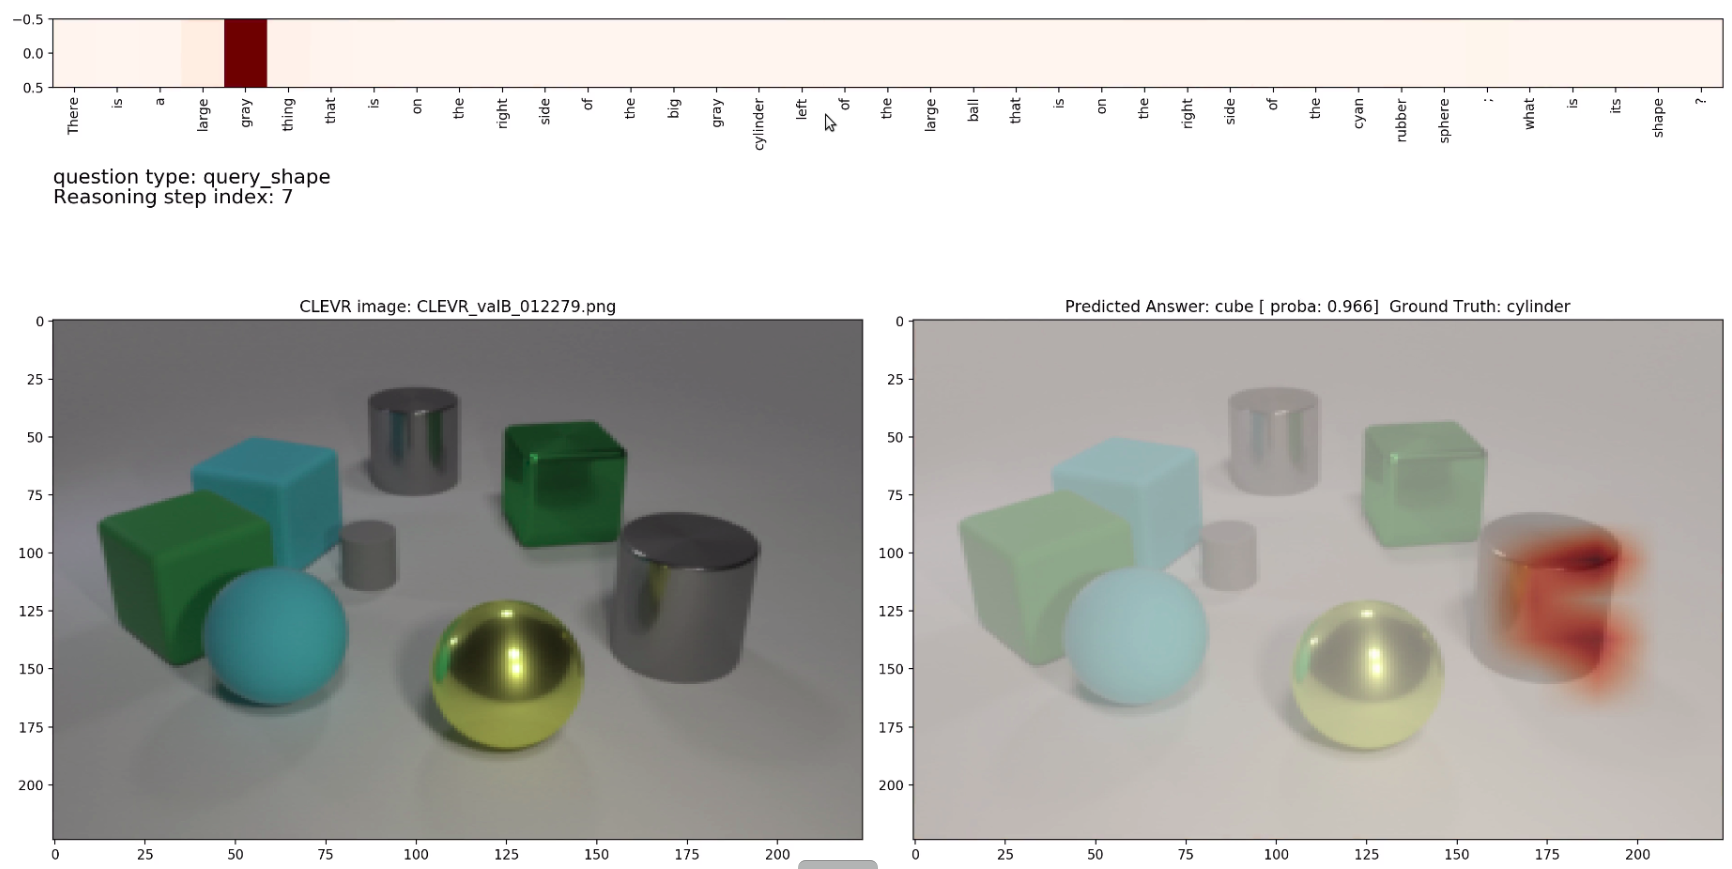
\includegraphics[width=\textwidth]{img/fail_mac_cogent_b_shape.png}
	\caption{The question reads as: \textit{There is a large gray thing that is on the right side of the big gray cylinder left of the large ball that is on the right side if the cyan rubber sphere; what is its shape?}}
	\label{fig:fail_mac_shape}
\end{figure}

\begin{figure}[]
	\centering
	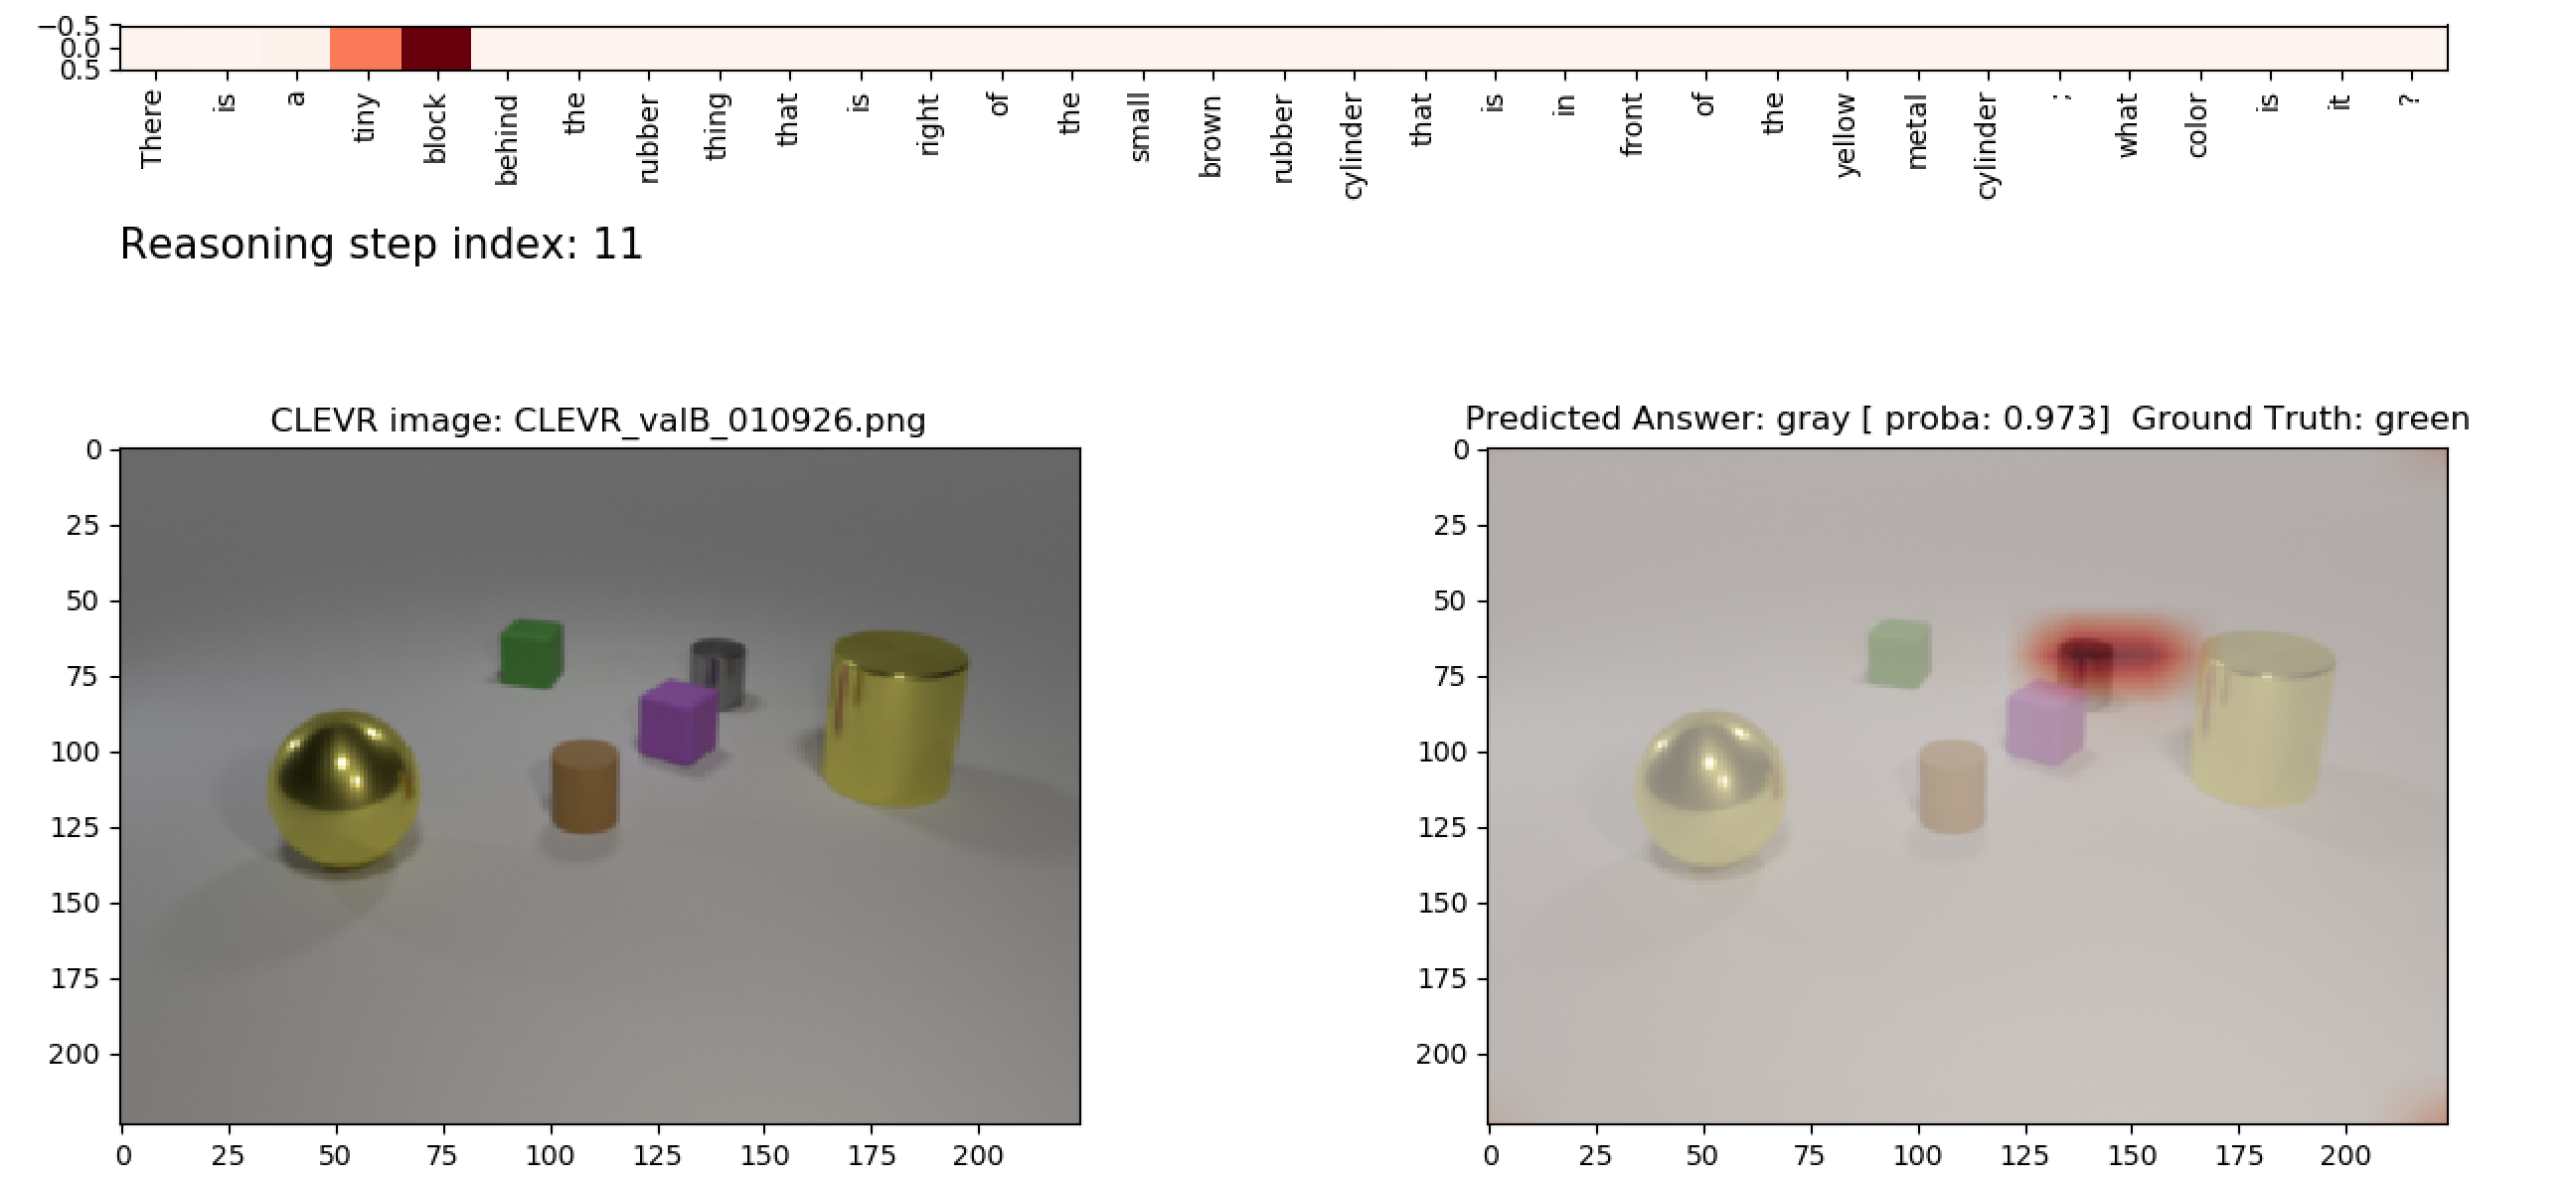
\includegraphics[width=\textwidth]{img/fail_mac_cogent_b_color.png}
	\caption{The question reads as: \textit{There is a tiny block behind the rubber thing that is right if the small brown rubber cylinder that is in front of the yellow metal cylinder; what color is it?}}
	\label{fig:fail_mac_color}
\end{figure}

Those examples indicate that MAC did not correctly separate the concept of shape from the concept of color, but have a better understanding of the colors (as it found the object of interest in \fig{fig:fail_mac_shape} by its color). This could come from that fact that the shape \textit{sphere} is associated with all possible colors in the dataset. 


\end{document}
